\Chapter{ETUDE THÉORIQUE}\label{sec:Theme1}
\begin{table}[htbp]
  \centering
  \caption{Constantes et variables des modèle analytiques}
  \begin{tabular}{|c|l|}
    \hline\rowcolor[gray]{0.8}\color{black}
    Symbole         & Description\\\hline
    $A$           & Aire de la section\\\hline
    $a$       & Rayon exeterne de la roue: $a=R+r_2$\\\hline
    $\delta$             & Flèche imposée par la force de compression\\\hline
    $E$           & Module d'Young du matériau\\\hline
    $E_{p,g}$          & Energie potentielle gravitationnelle\\\hline
    $E_{tot}$          & Energie mécanique totale\\\hline
    $F$             & Force de compression appliquée à la roue\\\hline
    $g$     & Accélération gravitationnelle\\\hline
    $H_{max}$          & Hauteur de saut maximale\\\hline
    $I$           & Moment quadratique de la section\\\hline
    $k$             & raideur équivalente de la roue\\\hline
    $k_1, k_2$           & Rayons de giration principaux de la roue\\\hline
    $m_r$          & Masse de la roue\\\hline
    $\Omega_0$           & Vitesse angulaire à laquelle la roue décrit des cercles (phase 1 du mouvement)\\\hline
    $\omega_0$           & Vitesse de rotation de la roue sur elle même lorsqu'elle roule (phase 1 du mouvement)\\\hline
    $R$       & Rayon médian de la roue\\\hline
    $r_1$ & Rayon interne de section pour une section circulaire\\\hline
    $r_2$             & rayon externe de section pour une section circulaire\\\hline
    $\theta_0$           & Angle d'inclinaison de la roue par rapport à la verticale en régime permanent\\\hline
    $r_c$           & Rayon des cercles obtenus par projection sur le sol du centre de gravité de la roue (phase 1)\\\hline
    $\rho$           & Masse volumique du matériau\\\hline
  \end{tabular}
  \label{tab:Definitions}
\end{table}


\section{Etude du saut d'une roue Cyr}
\subsection{Description du mouvement}
La roue Cyr est comprimée d'une flèche $\delta$ imposée par une force exercée selon l'axe de son diamètre par une force $F$ puis relâchée. Une partie de l'énergie de déformation élastique est transformée en saut. On notera $H_{max}$ la hauteur correspondant à l'énergie potentielle par laquelle s'élève le centre de gravité de la roue de sa position au repos à sa hauteur maximale.


\subsubsection{Hypothèses}
\begin{itemize}
    \item On considère que le support contre lequel la roue est comprimée est parfaitement rigide.
    \item On néglige la force de trainée de l'air.
    \item La répartition des masses est idéalisée
\end{itemize}

\subsubsection{Modèle deux degrés de liberté}
On modélise la roue Cyr par deux masses ponctuelles égales $\frac{m_r}{2}$ reliées par un ressort de longueur à vide $2R$, où $R$ correspond au rayon médian de la roue, et de rigidité $k$. \\
$k$ correspond à la constante élastique qui régit la relation $F=k \delta$, pour un anneau elle dépend du module d'Young $E$, du rayon médian $R$ et du moment quadratique de la section $I$: $k=\frac{4\pi EI}{(\pi^2 -8)R^3}$ \cite{yangkim}
\\
 Les positions des masses sont reperées par les ordonnées $y_1$ et $y_2$.

\begin{figure}[htb]
\centering
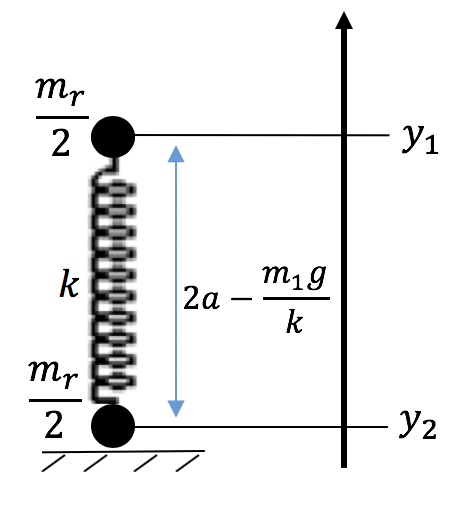
\includegraphics[width=2in]{images_2ddl/repos.png}
\caption{Système au repos}
\label{fig:repos}
\end{figure}

On note $t_0<0$ le moment auquel on relâche le ressort. $t=0$ correspond au moment auquel la masse inférieure quitte le sol, c'est à dire au moment où la force qui lui est transmise par le ressort devient suffisante pour prendre le dessus sur la gravité:$\frac{m_r g}{2}=k(y_1-2R)$. \\
Les positions des masses à $t=0$ sont donc $y_1=2R+\frac{m_r g}{2k}$ et $y_2=0$
On note $t_f$ le temps pour lequel le centre de gravité du système atteint sa hauteur maximale.

\begin{figure}[htb]
\centering
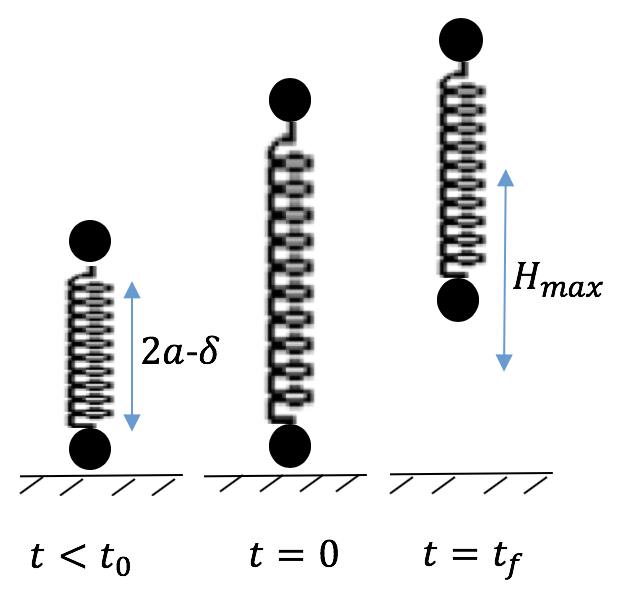
\includegraphics[width=3in]{images_2ddl/saut.png}
\caption{Saut du système}
\label{fig:saut}
\end{figure}

\subsection{Mise en équations}

Pour $t_0<t<0$, la masse 1 est soumise à deux forces de directions confondues avec l'axe du ressort: son propre poids de norme $-\frac{m_r g}{2}$, ainsi qu'à la force élastique de norme $-k(y_1-2R)$.
La relation fondamentale de la dynamique se traduit par le système d'équations \ref{eq:1}:

\begin{equation}
   t_0<t<0: 
  \begin{cases}
    \frac{m_r}{2}\frac{d^2y_1}{dt^2}+k(y_1-2R)+\frac{m_r}{2}g=0\\
    y_2=0 \\
    $y_1(t_0)=2R-\frac{F}{k}$
    $y_1(0)=2R+\frac{m_r g}{2k}$
  \end{cases}
  \label{eq:1}
\end{equation}


Pour $t_0<t<0$, le mouvement est donc régi par le système \ref{eq:2}:

\begin{equation}
  \begin{cases}
    \alpha_0=\sqrt{\frac{2k}{m_r}}\\
    y_1(t)=(\frac{m_r g}{2k}-\frac{F}{k})\cos(\alpha_0(t-t_0))-\frac{m_r g}{2k}+2R \\
    y_2=0
  \end{cases}
  \label{eq:2}
\end{equation}

La vitesse initiale de la masse 1 s'exprime $v_{10}=\alpha_0(\frac{m_r g}{2k}-\frac{F}{k})\sin{\alpha_0 t_0}$ \\

Or, comme $y_1(t_0)=2R-\frac{F}{k}$, on a $\cos{(\alpha_0 \t_0)}=\frac{2m_rg}{m_rg-2F}$ et donc $\sin{(\alpha_0 \t_0)}=\sqrt{1-(\frac{2m_rg}{m_rg-2F})^2}$ \\
D'où $v_{10}=\sqrt{\frac{4F^2 -3(m_r g)^2-4Fm_rg}{2 k m_r}}$

Lorsque $0<t<t_f$, les masses 1 et 2 sont chacune soumises à leur poids et à la force élastique due à la déformation du système.
La relation fondamentale de la dynamique appliquée aux masses 1 et 2 donne alors:

\begin{equation}
   0<t<t_f: 
  \begin{cases}
    \frac{m_r}{2}\frac{d^2y_1}{dt^2}+k(y_1-y_2-2R)+\frac{m_r}{2}g=0\\
    \frac{m_r}{2}\frac{d^2y_2}{dt^2}+k(y_2-y_1+2R)+\frac{m_r}{2}g=0
  \end{cases}
  \label{eq:3}
\end{equation}

Avec les conditions initiales: 
\begin{equation}
  \begin{cases}
    y_1(0)=2R+\frac{m_r g}{2k}\\
    \frac{d y_1}{dt}(0)=v_{10}=\sqrt{\frac{4F^2 -3(m_r g)^2-4Fm_rg}{2 k m_r}}\\
    y_2(0)=0 \\
    \frac{d y2}{dt}(0)=0
  \end{cases}
  \label{eq:4}
\end{equation}

En résolvant \ref{eq:3} on obtient les équations décrivant les mouvements des masses 1 et 2 pour $0<t<t_f$:

\begin{equation}
  \begin{cases}
    \alpha=\sqrt{\frac{4k}{m_r}}\\
    y_1(t)=\frac{1}{2}(-\frac{g t^2}{2}+v_{10}t+(\frac{m_r g}{2k})\cos{\alpha t}+\frac{v_{10}}{\alpha}\sin{\alpha t}+\frac{m_r g}{2k}+4R) \\
    y_2(t)=\frac{1}{2}(-\frac{g t^2}{2}+v_{10}t-(\frac{m_r g}{2k})\cos{\alpha t}-\frac{v_{10}}{\alpha}\sin{\alpha t}+\frac{m_r g}{2k}) 
  \end{cases}
  \label{eq:5}
\end{equation}

Ce qui nous donne les expressions temporelles de la variation de l'allongement du système et de l'évolution de la positon de son centre de gravité:

\begin{equation}
  \begin{cases}
    y_1(t)-y_2(t)= (\frac{m_r g}{2k})\cos{\alpha t}+\frac{v_{10}}{\alpha}\sin{\alpha t}+2R\\
    \frac{y_1(t)+y_2(t)}{2}=\frac{1}{2}(-\frac{g t^2}{2}+v_{10}t+\frac{m_2 g}{k} +2a)
  \end{cases}
  \label{eq:6}
\end{equation}

Ces équations permettent de tracer des animations du mouvement afin de mieux appréhender ce dernier par la suite. Tout au long de l'élévation du centre de gravité de la roue, on peut observer des déformations correspondant au second mode vibratoire d'un anneau (déformations planes).
\\ 
\\


Lorsqu'on arrive à $t=t_f$, la vitesse du centre de gravité s'annule. Il suffit alors de dériver l'expression de la position du centre de gravité déterminée ci-dessus pour obtenir: $t_f=\frac{v_{10}}{g}$, soit: 
$$ t_f=\sqrt{\frac{4F^2 -3(m_r g)^2-4Fm_rg}{2 k m_r g^2}}$$

On substitue ensuite cette expression à $t_f$ dans l'expression de la position du centre de gravité pour avoir la hauteur maximale de ce dernier, à laquelle on soustrait sa position à l'équilibre statique $y_{cdg,ref}=\frac{1}{2}(2R-\frac{m_r g}{2k})$ pour obtenir finalement l'expression de $H_{max}$.
\\ \\
Ainsi: $H_{max}=\frac{4F^2+(m_rg)^2-4Fm_rg}{8km_rg}$
\\

Ainsi, les paramètres influençant la hauteur maximale de saut du système sont:
\begin{itemize}
    \item La force de compression $F$ à laquelle ce dernier est soumis initialement
    \item La masse du système, déterminée par sa géométrie et la masse volumique du matériau
    \item La raideur équivalente du système qui dépend de sa géométrie et du module de Young du matériau.
\end{itemize}

L'expression de $H_{max}$ nous permet d'étudier l'efficacité énergétique du système, c'est à dire d'estimer quelle fraction de l'énergie totale fournie au système sous forme de déformation élastique est convertie en énergie potentielle gravitationnelle servant au saut. \\
Pour cela on s'intéresse au ratio $\frac{E_{p,g}}{E_{tot}}$ de ces deux quantités. \\
Avec $E_{tot}=\frac{F^2}{2k}$ et $E_{p,g}=m_r g H_{max}$, on obtient:  $\frac{E_{p,g}}{E_{tot}}=1-\frac{m_rg}{F}+\frac{(m_r g)^2)}{4F^2}$.

\subsection{Traitement numérique du modèle}
Dans la partie qui suit, on étudie pour chaque paramètre dont dépendent $H_{max}$ et le ratio d'efficacité énergétique comment ces derniers évoluent lorsqu'on fait varier un de ces paramètre indépendamment des autres.
\\ 
\\ 
La variation de ces paramètres doit respecter les valeurs limites suivantes, en dessous desquelles le modèle n'est plus valide:
\begin{itemize}
    \item Pour $F$: Pour que le modèle soit valide il faut qu’il y ait un saut, l'énergie de déformation élastique doit être suffisante pour faire décoller la masse 2, ce qui se traduit par: $\frac{1}{2} \frac{F^2}{k}>\frac{(m_r g)^2}{4k}$  soit: $F>\frac{m_r g}{\sqrt{2}}$
    \item Pour $k$: Le ressort doit pouvoir soutenir la masse 1: $\frac{m_r g}{2k}<2R$ c'est à dire: $k>\frac{m_r g}{4R}$ 
    \item Pour $m_r$: Diminuer $m_r$ revient à retirer de la matière, il y a donc une masse limite dépendant des propriétés mécaniques du matériau en dessous de laquelle il y aura rupture lors de la compression, la roue étant devenue trop fragile.
\end{itemize}
Les limites seront indiquées par des pointillés sur les tracés plus bas
\\
On applique le modèle développé dans la section précédente aux quatre cas suivants:
\begin{itemize}
	\item Une roue en acier dont les dimensions, détaillées en Figure~\ref{fig:geo1} ,  ont été mesurées sur une roue existante (cas témoin)
	\item Une roue en matériau composite de dimensions identiques à celles de la première
	\item Une roue en matériau composite de section elliptique dont le prolongement du petit axe coincide avec l'axe de révolution (cas 1), dont les dimensions sont détaillés Figure~\ref{fig:geo2}
	\item Une roue en matériau composite de section elliptique dont le prolongement du grand axe coincide avec l'axe de révolution (cas 2), dont les dimensions sont détaillés Figure~\ref{fig:geo2}
\end{itemize}

\begin{figure}[htb]
\centering
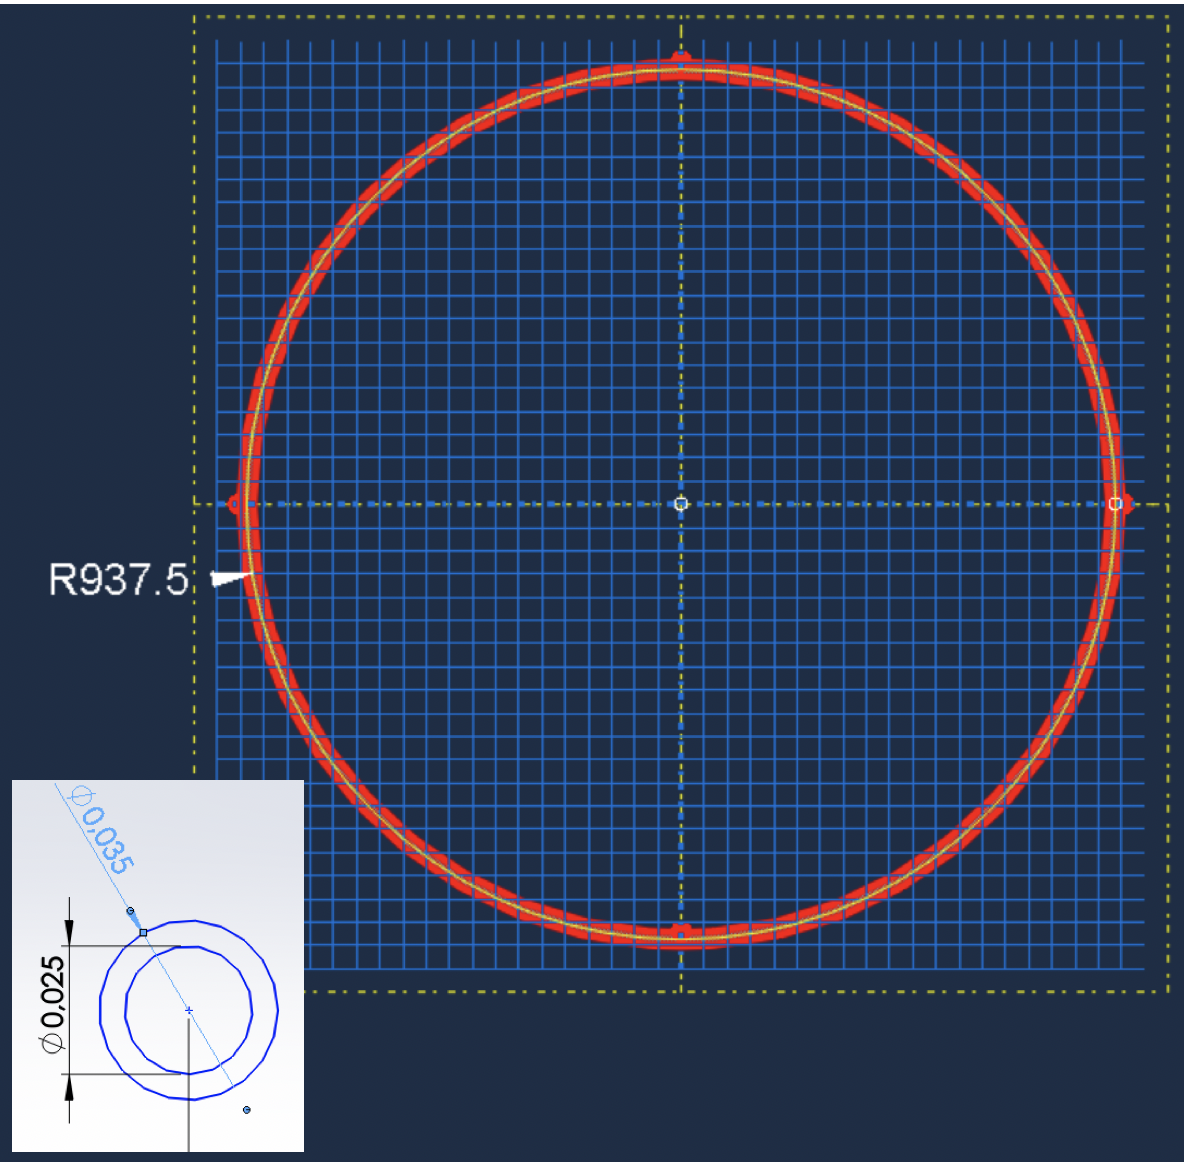
\includegraphics[width=4in]{images_2ddl/geo1.png}
\caption{Géométrie et dimension des roues Cyr à sections circulaires étudiées dans cette partie}
\label{fig:geo1}
\end{figure}

\begin{figure}[htb]
\centering
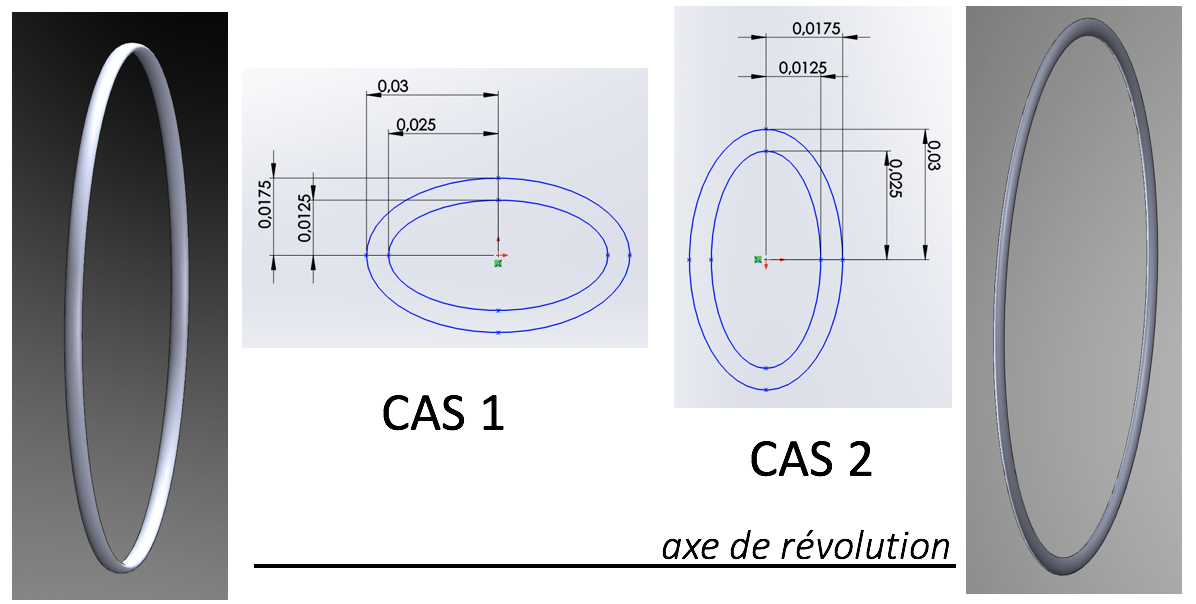
\includegraphics[width=4in]{images_2ddl/geo2.png}
\caption{Géométrie et dimension des roues Cyr à sections elliptiques étudiées dans cette partie}
\label{fig:geo2}
\end{figure}


Si on fait varier un paramètre indépendamment des autres, il est nécessaire d'affecter une valeur à ces derniers, fixés momentanément:
\begin{itemize}
	\item Les géométries considérées sont celles présentées en  Figures \ref{fig:geo1} et \ref{fig:geo2}
	\item On considère que la force $F$ appliquée au système a pour norme $900 N$, correspondant au poids d'un athlète se suspendant à une main à la roue.
	\item Les propriétés mécaniques de l'acier sont les suivantes $E_a=210GPa$, $\rho_a=7800 kg m^-3$
	\item Pour le matériau composite, on considère dans un premier temps qu'il s'agit d'une matrice nylon renforcée de fibres de carbones courtes, qu'on considère isotrope. On a donc: $E_c=9 GPa$, $G=3.8 GPa$, $\rho_c=1170 kg m^-3$, avec une contrainte à la rupture $\sigma_r=63 MPa$
\end{itemize}
Dans ce qui suit, lorsqu'on fait varier une seul paramètre, les autres, momentanément fixés, prennent les valeurs qui leur ont été attribuées ci-dessus.
\\
\\ 
Premièrement, avec ces données il est possible de déterminer la masse minimale que devra avoir la roue (on considère le cas d'une section circulaire):
\begin{itemize}
    \item On commence par calculer les contraintes lorsque la roue est comprimée par une force $F$: La contrainte dans l'arrête extérieure s'exprime $\sigma_i=k_i\sigma$ \cite{roark},
    où sigma est la contrainte calculée pour une poutre droite: $\sigma=\frac{Mr_2}{I_z}$, avec $I_z=\frac{\pi}{2}(r_2^4-r_1^4)$ et $M=\frac{\pi}{4}FR$.
    D'après les formules du livre de Roark, $k_i$ s'exprime $k_i=\frac{1}{4\beta}\frac{1-\beta}{\frac{R_c}{r_2}-1}[1+(\frac{r_1}{r_2})^2]$ avec $\beta=\frac{1}{2}[\frac{2R_c}{r_2}-\sqrt{(\frac{R_c}{r_2})^2-1}-\sqrt{(\frac{R_c}{r_2})^2-(\frac{r_1}{r_2})^2}]$ 
    \item Il ne reste plus qu'à déterminer le rayon de courbure de la roue comprimée, comme illustré sur la figure \ref{fig:ellr}: $R_c=\frac{a_r^2}{b_r}$, $a_r$ et $b_r$ étant respectivement les demi grand axe et demi petit axe de l'ellipse que devient la roue lorsqu'elle est comprimée.\\
    
    \begin{figure}[htb]
    \centering
    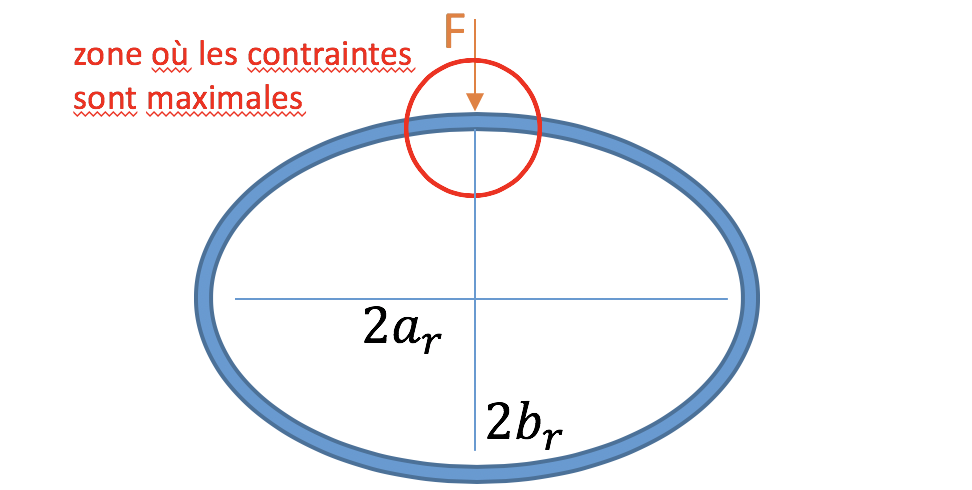
\includegraphics[width=4in]{images_2ddl/ellr.png}
    \caption{}
    \label{fig:ellr}
    \end{figure}
    
\begin{itemize}
    \item Pour calculer $a_r$ et $b_r$, on utilise les formules du livre de Roark qui donnent les variations de diamètre horizontal $\Delta D_h$ et vertical $\Delta D_v$ d'une anneau comprimé selon son diamètre avec une force $F$, et on aura ainsi $a_r=R+\frac{\Delta D_h}{2}$ et $b_r=R+\frac{\Delta D_v}{2}$.
    \item D'après les formules de Roark, $\Delta D_h=\frac{FR^3}{EI}(\frac{1}{2}(1+\frac{I}{AR^2}+\frac{2EI}{GAR^2})-1+\frac{2}{/pi}(1-\frac{I}{AR^2})^2)$ et $\Delta D_v=-\frac{FR^3}{EI}(\frac{\pi}{4}(1-\frac{I}{AR^2}+\frac{2EI}{GAR^2})-\frac{2}{/pi}(1-\frac{I}{AR^2})^2)$, où $A$ est l'aire de section, $E$, le module de Young, $G$, le module de cisaillement, $R$, le rayon médian de la roue, et $I$ le moment de section quadratique selon l'axe principal perpendiculaire au plan de la roue.
    \item En implémentant numériquement les équations ci-dessus, on est capable de calculer les contraintes maximales auxquelles sera soumise la roue pour une force de compression $F$ donnée. Pour $F=900N$, en fixant $r_2$ et en faisant varier $r_1$ de $0$ à $r_2$, on est capable de tracer les contraintes maximales, en fonction de la masse de la roue, $m_r=2\pi\rho A R$. Comme l'illustre la figure-\ref{fig:mmin1} ci-dessous, il est alors possible de déterminer la masse à partir de laquelle les contraintes passent sous le seuil de $63 MPa$, et donc à partir de laquelle il y a rupture.
    
\end{itemize}


\begin{figure}[htb]
\centering
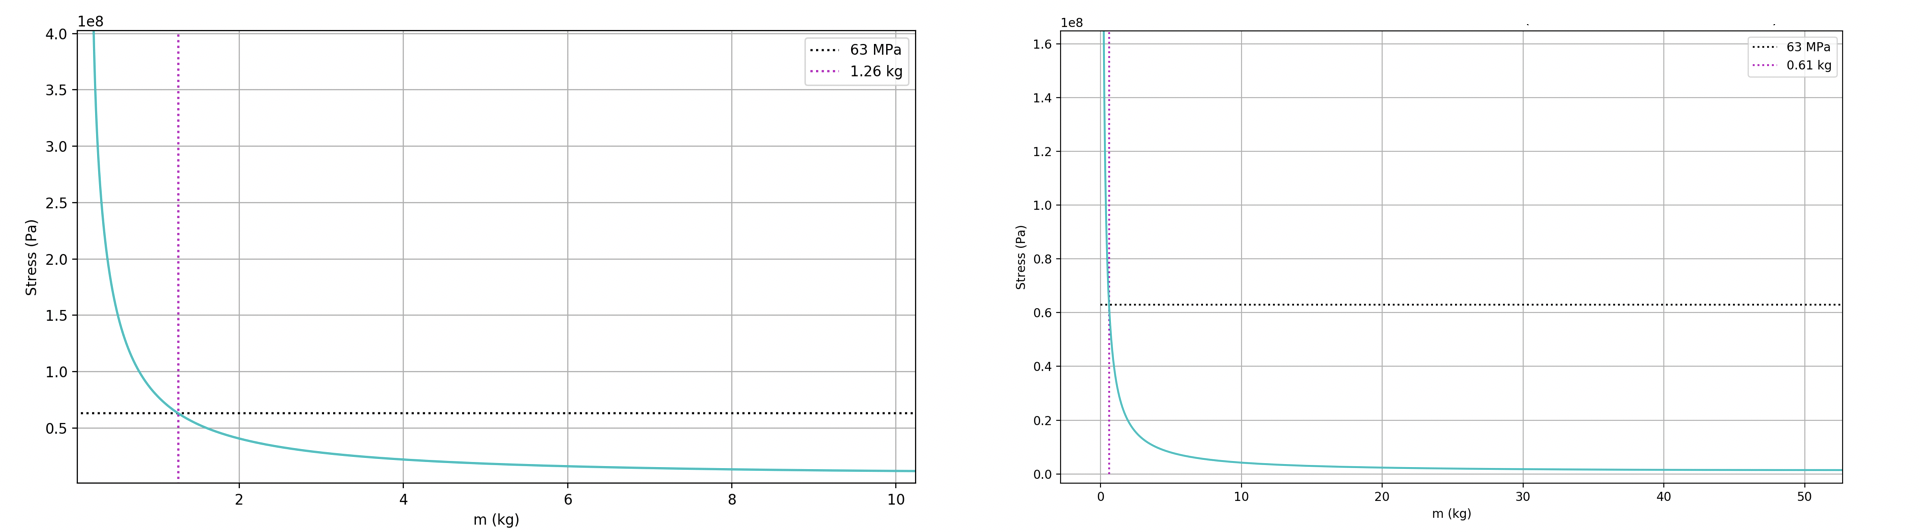
\includegraphics[width=7in]{images_2ddl/mmin1.png}
\caption{Contraintes maximales dans la roue en fonction de sa masse, pour $r_2=2.5 cm$ et $r_1$ variant de $0.0$ à $2.49 cm$ (gauche) et $r_2=5.0 cm$ et $r_1$ variant de $0.0$ à $4.99 cm$}
\label{fig:mmin1}
\end{figure}


\begin{itemize}
    \item On peut donc implémenter ce procédé numériquement pour déterminer cette valeur minimale de la masse pour en fonction de $r_2$. Le resultat de l'implémentation est présenté à la figure-\ref{fig:mmin2} ci-dessous. 
\end{itemize}


\begin{figure}[htb]
\centering
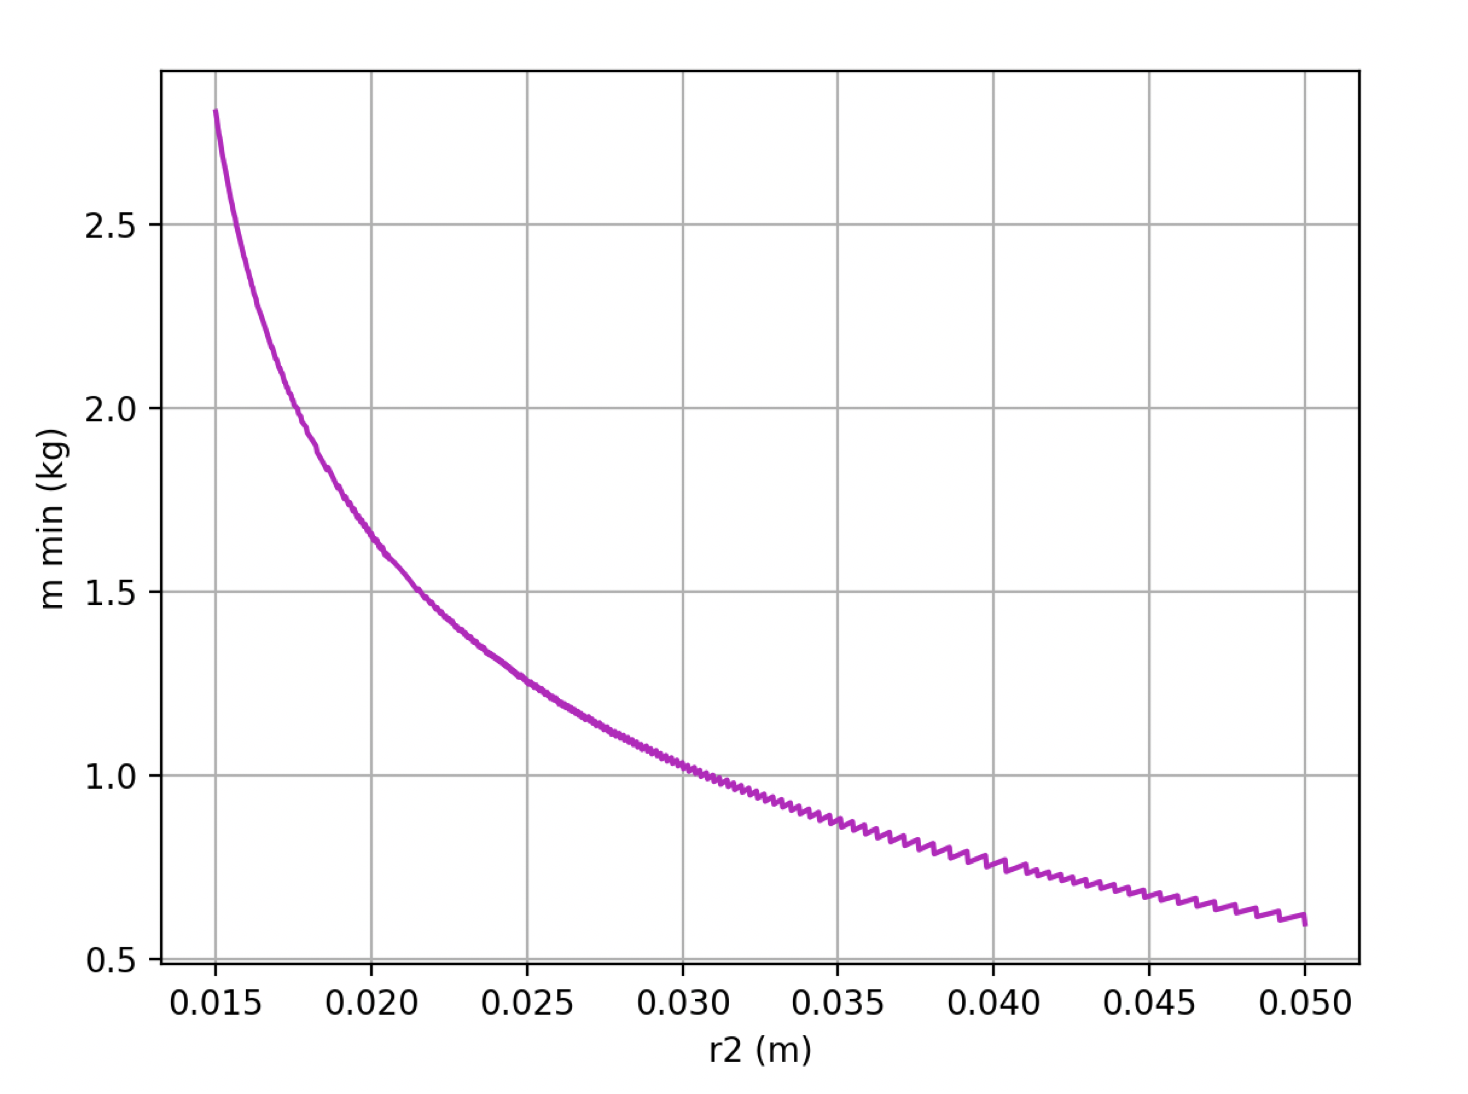
\includegraphics[width=4in]{images_2ddl/mmin2.png}
\caption{Masse minimale de la roue en fonction de $r_2$}
\label{fig:mmin2}
\end{figure}


\item Pour ce qui suit, $r_2$ sera fixé à $1.75 cm$, la masse minimale sera donc $2.0 kg$

\end{itemize}

\begin{figure}

  \begin{subfigure}
  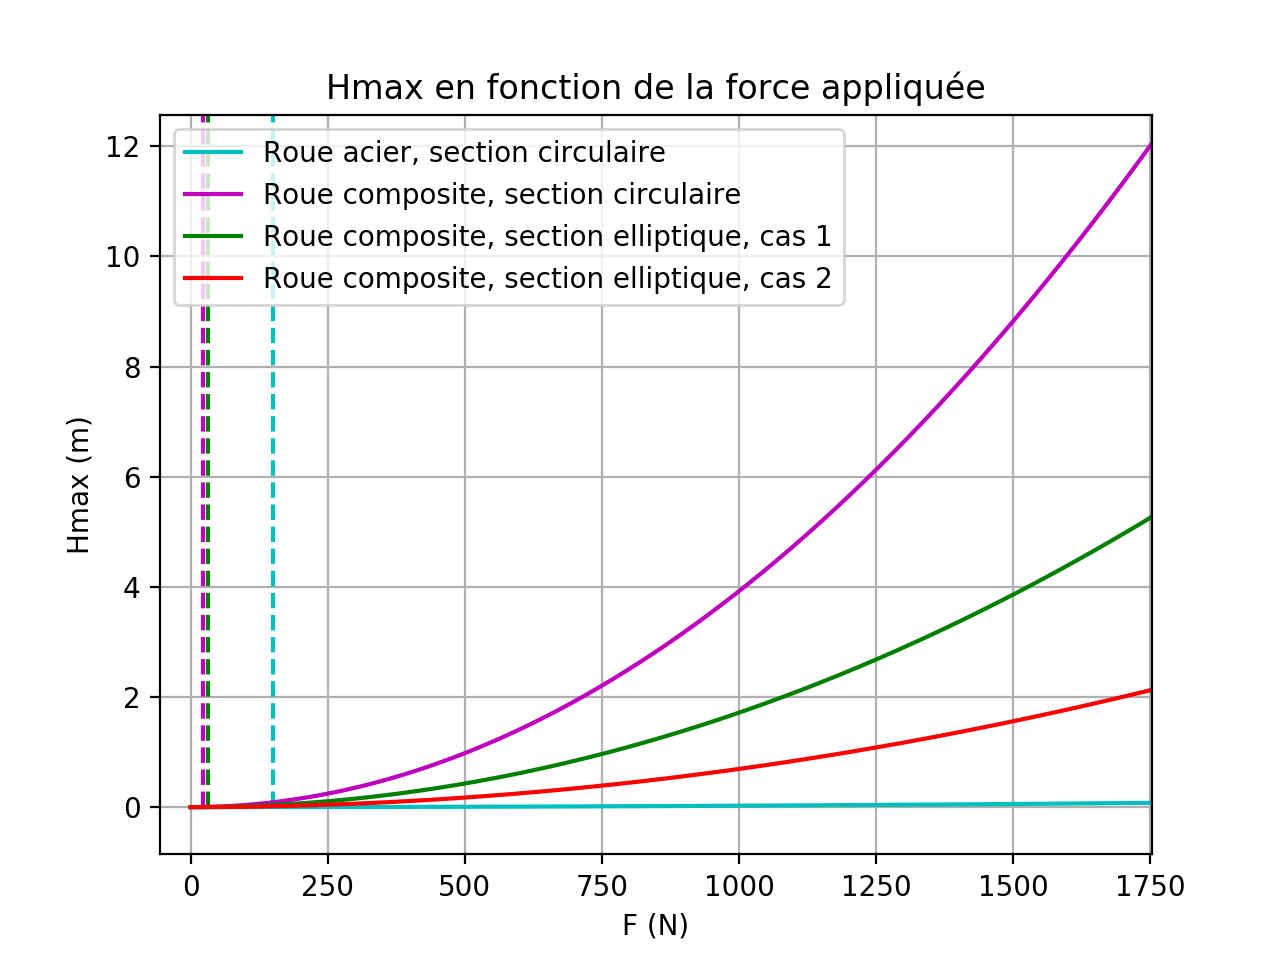
\includegraphics[width=3in]{images_2ddl/hmaxf.png}
  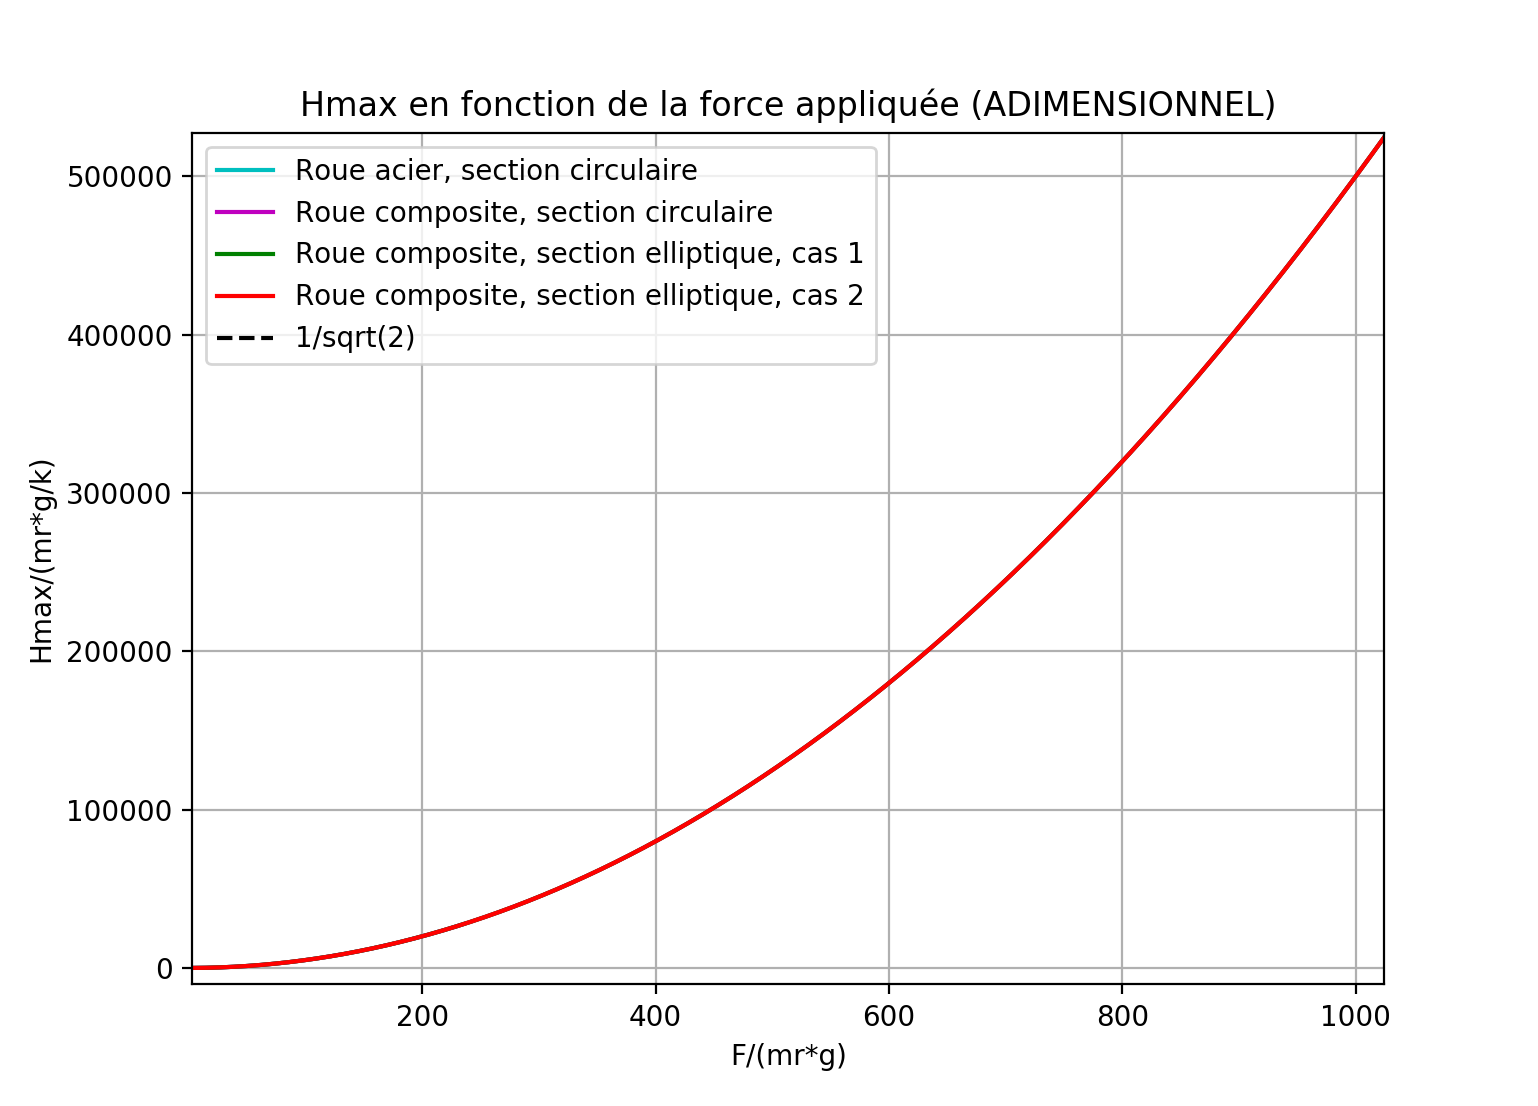
\includegraphics[width=3in]{images_2ddl/hmaxfa.png}
  \end{subfigure}
  \begin{subfigure}
  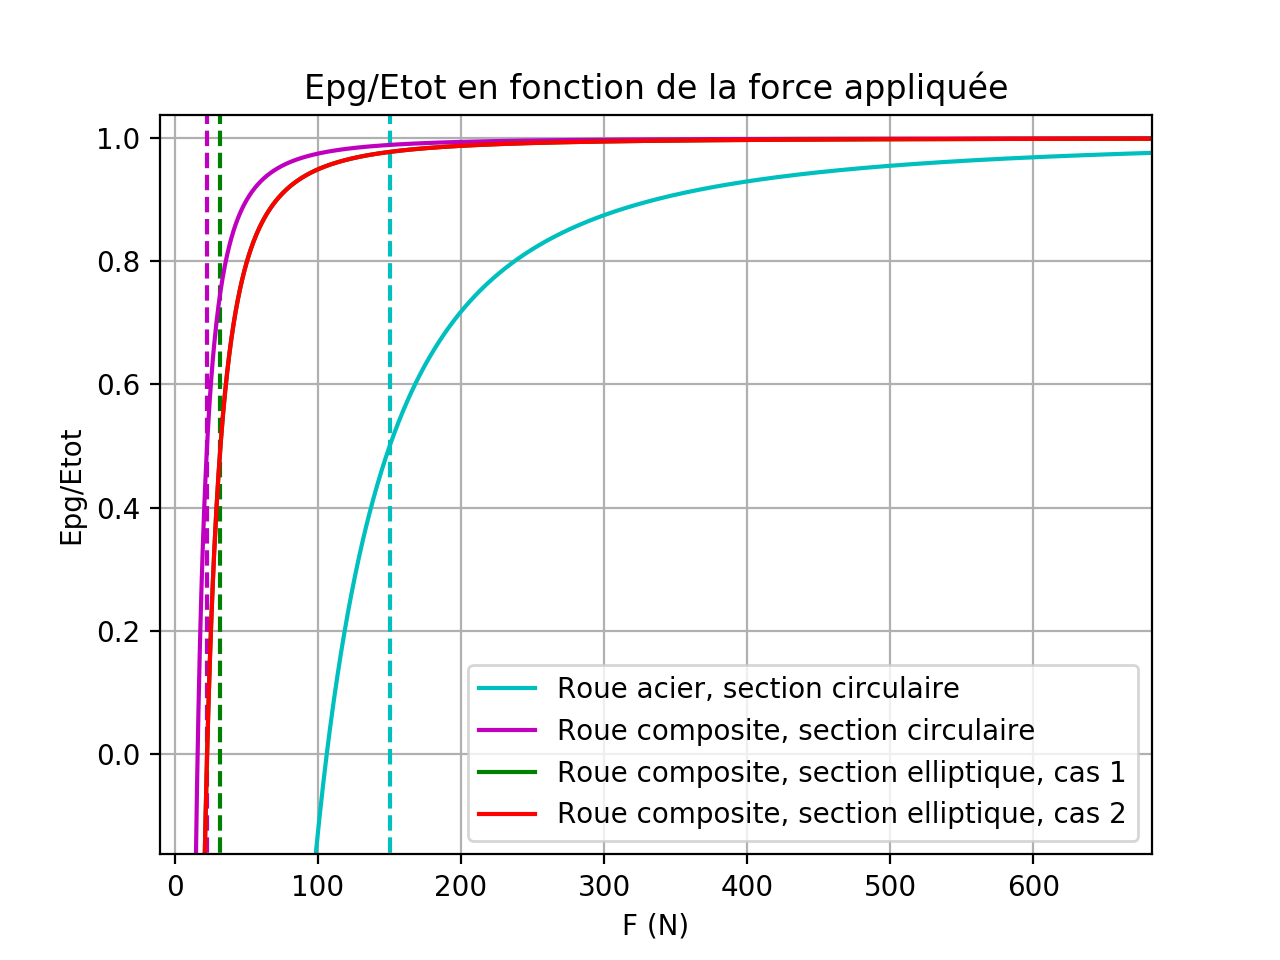
\includegraphics[width=3in]{images_2ddl/epf.png}
  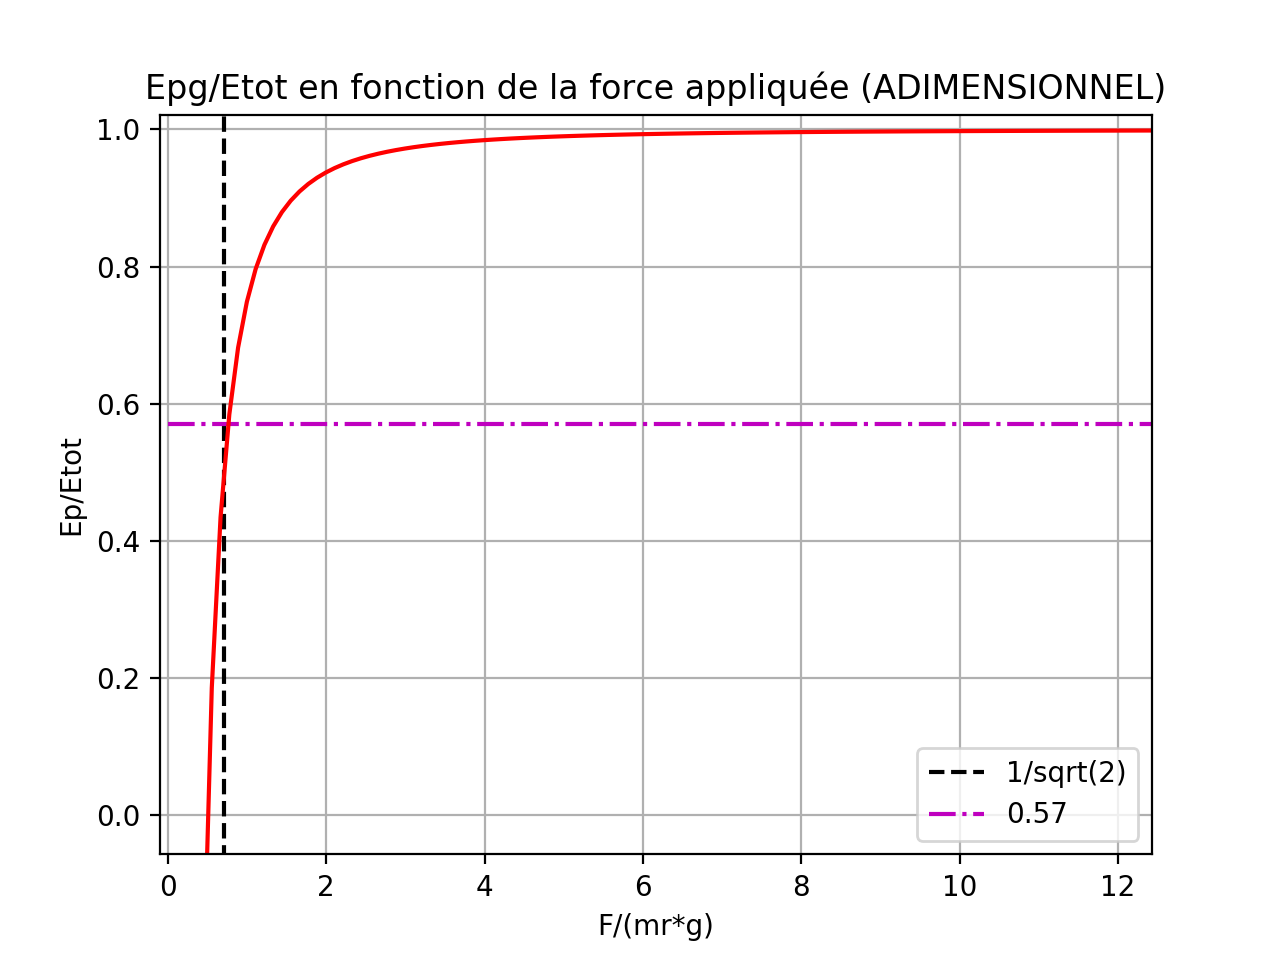
\includegraphics[width=3in]{images_2ddl/epfa.png}
  \end{subfigure}
  \begin{subfigure}
  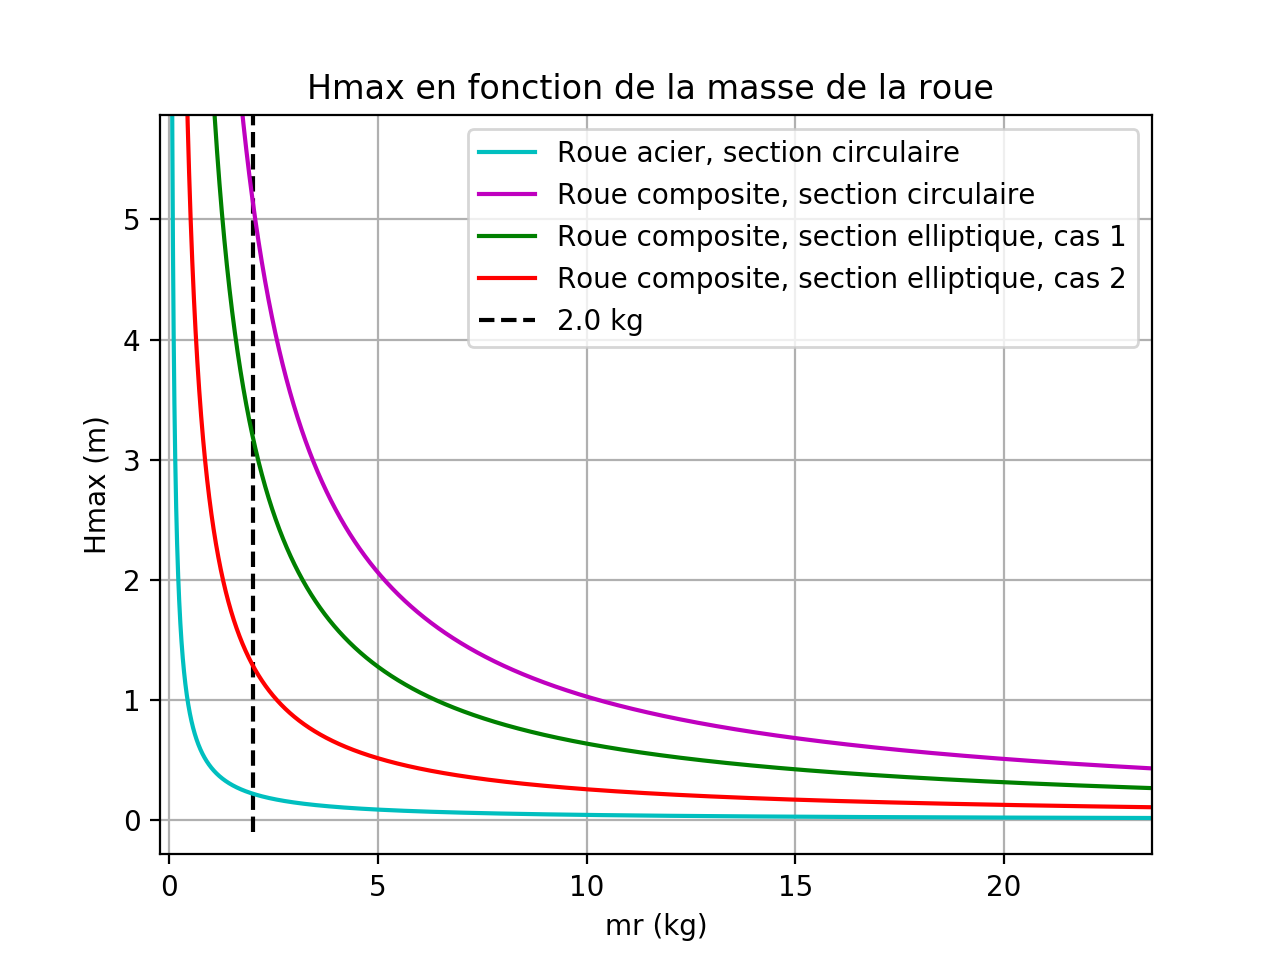
\includegraphics[width=3in]{images_2ddl/hmaxm.png}
  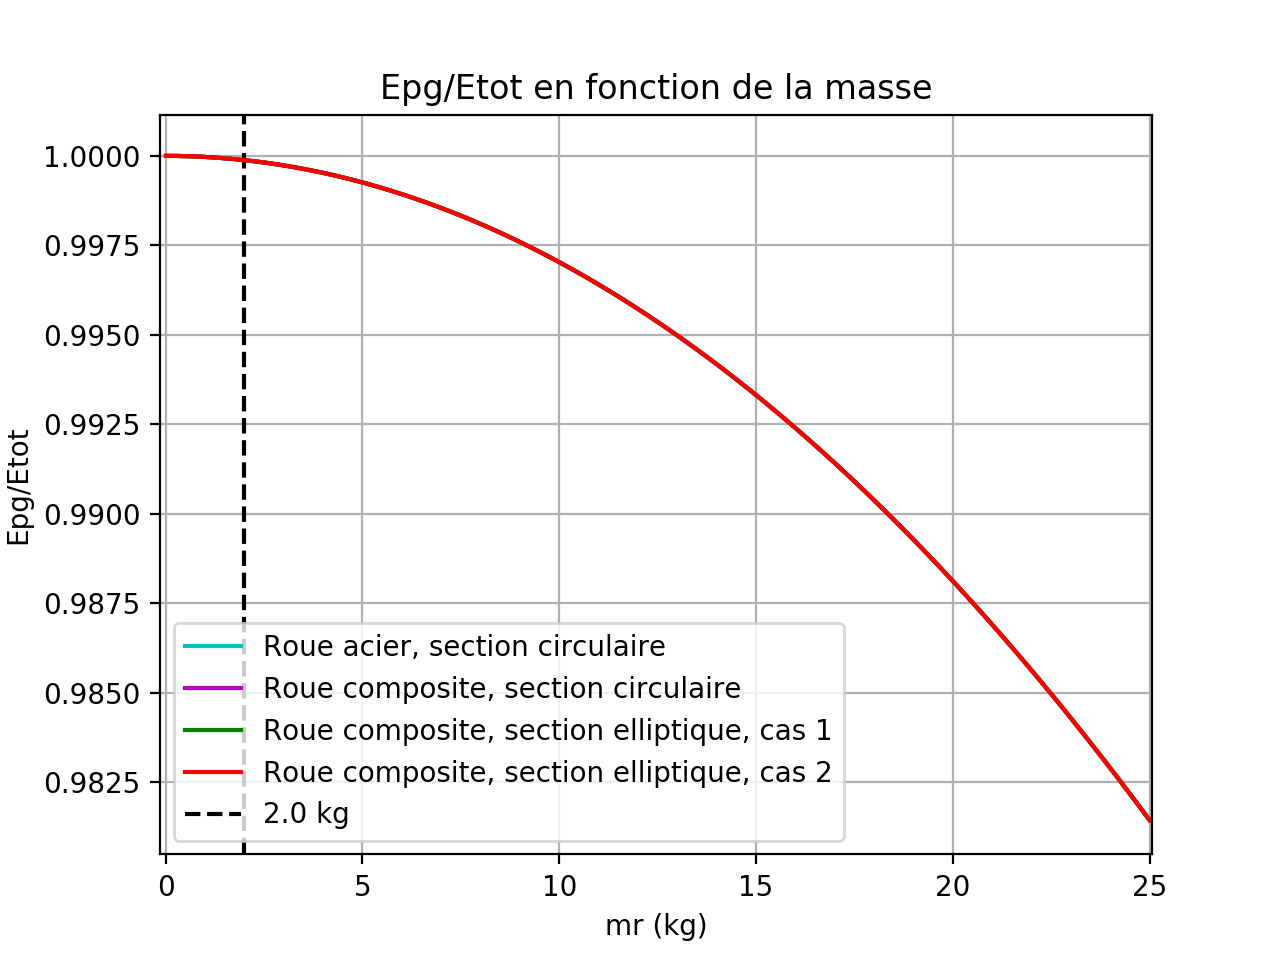
\includegraphics[width=3in]{images_2ddl/epm.png}
  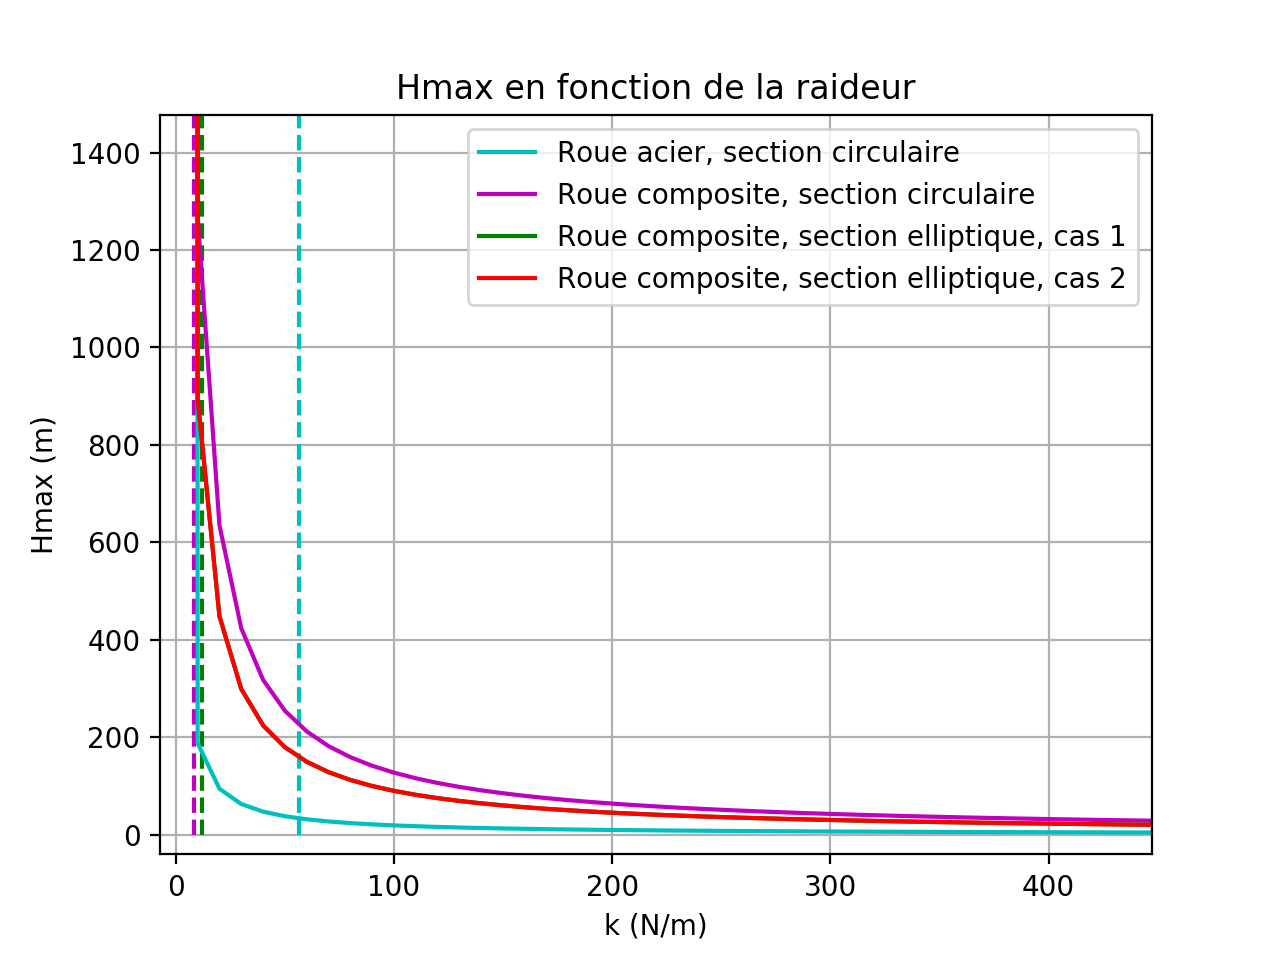
\includegraphics[width=3in]{images_2ddl/hmaxk.png}
  \end{subfigure}
  
  \caption{Variations de $H_{max}$ et de $\frac{E_{p,g}}{E{tot}}$}
\end{figure}



Remarques:
\begin{itemize}
    \item Les tracés adimensionnels permettent d'étudier une tendance globale, ainsi que de s'affranchir de la dépendance des résultats avec les autres paramètres.
    \item Pour les roues composites définies plus haut, et le modèle étudié présentement, le rendement énergétique atteint un pallier à partir d'une certaine force ($F \sim 500 N$ dans notre cas )
    \item Pour une force $F=900 N$ imposée, une variation de la masse du système n'influe que légèrement sur l'efficacité énergétique (sa valeur la plus basse est environ 75$\%$, ce qui est acceptable) . La force appliquée à la roue est le paramètre déterminant pour cette dernière. Dans la continuité de cette observation, l'accentuation de la pente $\frac{H_{max}}{F}$, croissante avec la force, traduit une "rentabilité" de l'énergie d'autant meilleure que la force qu'on applique est élevée.
    \item Pour avoir un rendement énergétique correct, le poids de la roue doit être inférieur à la moitié de la norme de la force de compression $F$
    \item A l'inverse, la courbe $H_{max}=f(k)$ s'aplatit rapidement à mesure que la raideur augmente. Il s'agit de trouver un compromis entre la solidité et la maximisation de la hauteur de saut.
\end{itemize}


\section{Stabilité dynamique du mouvement}
\subsection{Description du mouvement}
On étudie ici le second mouvement caractéristique de la roue Cyr, analogue au mouvement du disque d'Euler. Le mouvement se découpe en deux phases, une première phase au cours de laquelle la roue décrit des cercles en roulant sur sa tranche, puis une deuxième phase où elle oscille en tournant de plus en plus vite avant de tomber à plat, stoppant net le mouvement. Ces deux phases correspondent à l'énchainement de deux figures de roue Cyr, la "roue" pour la phase 1 et la pièce pour la phase 2. \\
Ce qui suit est basé sur l'article de Batista \cite{Batista}, dont la démarche et le modèle mathématique développés pour le disque d'Euler ont été adaptés à la géométrie torique de la roue Cyr. De même que Batista, l'objectif est de développer des cartes de stabilité dynamiques, avec d'autres variables adaptées à notre cas.

\subsection{Hypothèses}
\begin{itemize}
    \item On se place en régime stationnaire: les variables qui prennent ainsi des valeurs constantes seront indicées d'un 0.
    \item On considère que la roue évolue sur un sol rugueux: il n'y a pas de glissement au niveau du point de contact.
    \item Le mouvement est étudié pour des valeurs de $\theta_0$ strictement comprises entre 0 et $\pi/2$ radians.
\end{itemize}

\subsection{Mise en équations}
\subsubsection{Variables et systèmes de coordonnées}

\begin{table}[htbp]
  \centering
  \caption{Constantes et variables des modèle analytiques}
  \begin{tabular}{|c|l|}
    \hline\rowcolor[gray]{0.8}\color{black}
    Symbole         & Description\\\hline
    $C$             & Centre de gravité de la roue\\\hline
    $P$             & Point de contact entre la roue et le sol\\\hline
    $A$             & Point autour duquel la roue roule en dessinant des cercles\\\hline
    $a$             & Rayon externe de la roue\\\hline
    $R$             & Rayon médian de la roue\\\hline
    $r_c$             & Rayon des cercles dessinés par la roue, obtenus par projection du centre de masse au sol\\\hline
    $(X_C,Y_C,Z_C)$           & Position du centre de gravité dans le reférentiel OXYZ\\\hline
    $(\psi,\theta,\phi)$       & Position angulaire de la roue dans OXYZ\\\hline
    $(v_{Cx},v_{Cy},v_{Cz})$           & Composantes de la vitesse du point C dans C{xzy} \\\hline
    $(\omega_1,\omega_2,\omega_3)$          & Composantes de la vitesse angulaire $\vec{omega}$ dans $C{\xi \eta \zeta}$\\\hline
    $\Omega$          & Vitesse angulaire par rapport à l'axe Z\\\hline
    $(F_x,F_y,F_z)$          & Composante de la force de réaction au point $P$ dans $C_{xzy}$ \\\hline
    $(M_x,M_y,M_z)$          & Composante du moment de réaction au point $P$ dans $C_{xzy}$ \\\hline
    $\Omega$          & Vitesse angulaire par rapport à l'axe Z\\\hline
  \end{tabular}
  \label{tab:batista}
\end{table}

On reprend les trois référentiels utilisés par Batista: $OXYZ$, $C{xzy}$ et $C{\xi\eta\zeta}$:

\begin{figure}[htb]
\centering
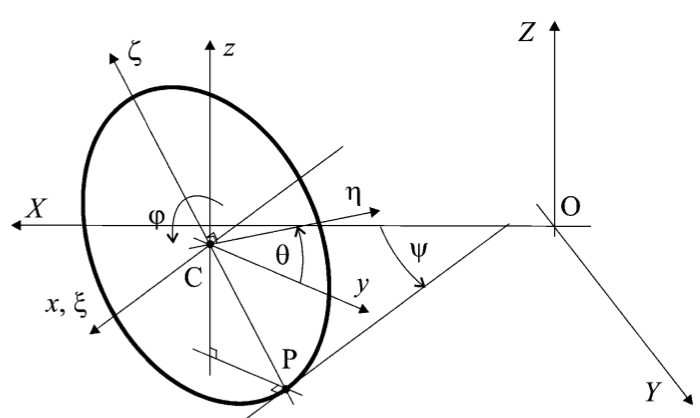
\includegraphics[width=4in]{batista/ref1.png}
\caption{Système de coordonnés, tiré de l'article de Batista \cite{Batista}}
\label{fig:ref1}
\end{figure}

\begin{figure}[htb]
\centering
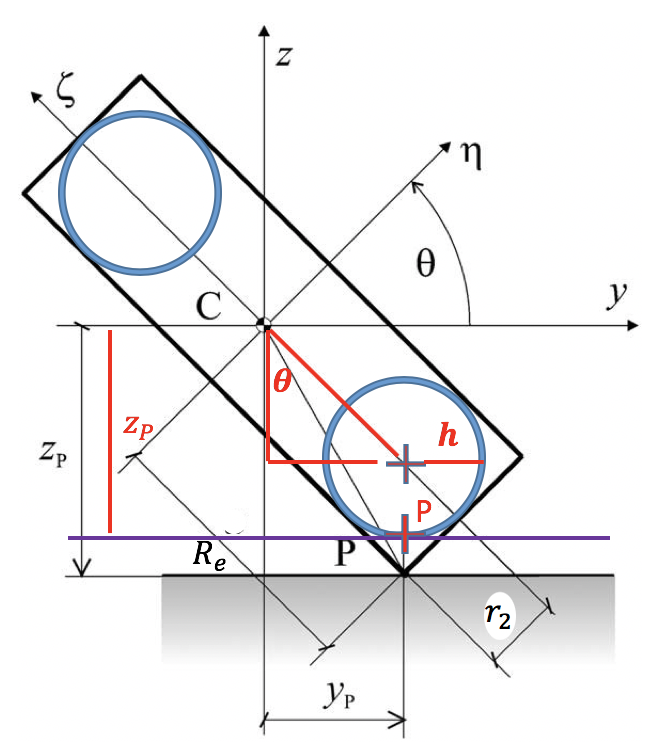
\includegraphics[width=4in]{batista/ref2.png}
\caption{Système de coordonnés, adapté de l'article de Batista \cite{Batista}}
\label{fig:ref2}
\end{figure}

\subsubsection{Equations}
Le mouvement de la roue est régie par les équations cinématiques suivantes \cite{Batista}:
\begin{equation}
  \begin{cases}
    \frac{dX_C}{dt}=v_{Cx0} \cos{\psi}- v_{Cy0} \sin{\psi}\\
    \frac{dY_C}{dt}=v_{Cx0} \sin{\psi}- v_{Cy0} \cos{\psi}\\
    \frac{dZ_C}{dt}=v_{Cz0} \\
    \frac{d\psi}{dt}=\Omega_0=\frac{\omega_{30}}{\cos{\theta_0}}\\
    \frac{d\theta}{dt}=\omega_{10}=0\\
    \frac{d\phi}{dt}=\omega_{20}-\omega_{30} \tan{\theta_0}
  \end{cases}
  \label{eq:b1}
\end{equation}


Les coordonnées du point de contact P dans C{xzy}, schématisé dans la figure \ref{fig:geo2} s'expriment:
\begin{equation}
  \begin{cases}
    x_P=0\\
    y_P=(a-r_2)\sin{\theta_0}=R\sin{\theta_0}\\
    z_P=-(a-r_2)\cos{\theta_0}-r_2=-R\cos{\theta_0}-r_2\\
  \end{cases}
  \label{eq:b2}
\end{equation}

D'après la règle de transport des torseurs, la vitesse du point de contact dans $C_{xzy}$ s'écrit:
\begin{equation}
    \vec{v_{P0}}=\vec{v_{C0}}+\vec{\omega_0} \wedge \vec{CP}
  \label{eq:b3}
\end{equation}

Les composantes de la vitesse au point de contact dans $C_{xzy}$ s'écrivent donc:
\begin{equation}
  \begin{cases}
    v_{Px_0}=v_{Cx_0}-\omega_{20} (R\cos{\theta_0}+r_2) -\omega_{30} R\sin{\theta} \\
    v_{Py_0}=v_{Cy_0} + \omega_{10} (R\cos{\theta_0}+r_2)= v_{Cy_0}\\
    v_{Pz_0}=v_{Cz_0} + \omega_{10} R\sin{\theta_0} = v_{Cz_0}
  \end{cases}
  \label{eq:b4}
\end{equation}

On a fait l'hypothèse d'un sol rugueux: on a donc $v_{Px0}=v_{Py0}=0$, et comme le contact entre le sol et la roue est permanent, $v_{Pz0}=0=v_{Cz_0}$.


Les composantes de l'accélération du centre d'inertie de la roue dans $C{xzy}$ s'expriment à partir de l'équation \ref{eq:b1} projetée dans $C{xzy}$:

\begin{equation}
  \begin{cases}
    a_{Cx0}=\frac{dv_{Cx0}}{dt}-\Omega_0 v_{Cy0}=-\Omega_0 v_{Cy0} \\
    a_{Cy0}=\frac{dv_{Cy0}}{dt} + \Omega_0 v_{Cx0}=\Omega_0 v_{Cx0}\\
    a_{Cz0}=\frac{dv_{Cz0}}{dt} = 0
  \end{cases}
  \label{eq:b5}
\end{equation}

Le moment cinétique au centre de masse s'exprime $\vec{L_C0}=I \cdot \vec{\omega}$, avec pour tenseur d'inertie:
$$
I=
\begin{pmatrix}
   m_r (\frac{1}{2}R^2+\frac{5}{8}r_2^2) & 0  &  0 \\
  0 &  m_r(R^2+\frac{3}{4}r_2^2) & 0 \\
  0 & 0 & m_r (\frac{1}{2}R^2+\frac{5}{8}r_2^2)
\end{pmatrix}
$$

Notons $k_1^2=\frac{1}{2}R^2+\frac{5}{8}r_2^2$ et $k_2^2=R^2+\frac{3}{4}r_2^2$

Les composantes du moment cinétique dans $C_{\xi \eta \zeta}$ s'écrivent donc:
\begin{equation}
  \begin{cases}
    L_{C\xi 0}=m_r k_1^2 \omega_{10}=0 \\
    L_{C\eta 0}=m_r k_2^2 \omega_{20}\\
    L_{C\zeta 0}=m_r k_1^2 \omega_{30}
  \end{cases}
  \label{eq:b6}
\end{equation}


Les relations fondamentales de la dynamique en translation et en rotation donnent alors:
\begin{equation}
  \begin{cases}
    m_r\Omega_0 v_{Cy0}=-F_x \\
    m_r \Omega_0 v_{Cx0}=F_y\\
    m_r(\frac{dv_{Cz0}}{dt})=-mg+F_z=0
  \end{cases}
  \label{eq:b7}
\end{equation}


\begin{equation}
  \begin{cases}
    m_r(k_2^2\omega_{20}-k_1^2\omega_{30} \tan{\theta_0})\omega_{30} +(R\cos{\theta_0}+r_2)F_y + R\sin{\theta_0}F_z + M_x =0\\
    -aF_x + M_y \cos{\theta_0} +M_z \sin{\theta_0}=0\\
    m_r(-k_2^2\omega_{20}+k_1^2\omega_{30} \tan{\theta_0})\omega_{10} + hF_x - M_y \sin{\theta_0} +M_z \cos{\theta_0}=0
  \end{cases}
  \label{eq:b8}
\end{equation}

La dérivée de l'énergie mécanique s'exprime: 
$$
\frac{dE}{dt}=P_F + P_M
\frac{dE}{dt}=\vec{v_P} \cdot \vec{F} + \vec{\omega} \cdot \vec{M}
$$

On étudie ici le régime stationnaire: les puissances de la force et du moment de réaction doivent être nulles. \\
Comme on a fait l'hypothèse du sol rugueux, on a déjà $\vec{v_P}=\vec{0}$. \\
Le disque doit avoir une vitesse de rotation pour qu'il y ait un mouvement à étudier, on a donc $\vec{M}=\vec{0}$

Les systèmes d'équations \ref{eq:b7} et \ref{eq:b8} deviennent alors:

\begin{equation}
  \begin{cases}
    F_y=m_r \Omega_0 v_{Cx0} \\
    m_r(k_2^2\omega_{20}-k_1^2\omega_{30} \tan{\theta_0})\omega_{30} +(R\cos{\theta_0}+r_2)m_r \Omega_0 v_{Cx0} + R\sin{\theta_0}mg =0
  \end{cases}
  \label{eq:b9}
\end{equation}

Or, on sait de l'équation \ref{eq:b1} que:

\begin{equation}
  \begin{cases}
    \omega_{20}=\omega_0 + \Omega_0 \sin{\theta_0}
    \omega_{30}=\Omega_0 \cos{\theta_0}
  \end{cases}
  \label{eq:b10}
\end{equation}

Et de l'équation \ref{eq:b2} que:\\
$v_{Cx0}=(R+r_2)\omega{20}-r_2\omega{30}$, c'est à dire $v_{Cx0}=(R+r_2)(\omega_0 + \Omega_0 \sin{\theta_0})-r_2\Omega_0 \cos{\theta_0}$

Ce qui donne:

\begin{equation}
 \begin{split}
     m_r(k_2^2(\omega_0 + \Omega_0 \sin{\theta_0})-k_1^2(\Omega_0 \cos{\theta_0}) \tan{\theta_0})(\Omega_0 \cos{\theta_0})\\
    +(R\cos{\theta_0}+r_2)m_r \Omega_0 ((R+r_2)(\omega_0 + \Omega_0 \sin{\theta_0})-r_2\Omega_0 \cos{\theta_0}) + R\sin{\theta_0}m_r g =0
 \end{split}
  \label{eq:b11}
\end{equation}

soit

\begin{equation}
 \begin{split}
     [(k_2^2-k_1^2)\sin(\theta_0)\cos(\theta_0)+(R \cos(\theta_0)+r_2)[(R+r_2)\sin(\theta_0)-r_2 \cos(\theta_0)]]\Omega_0^2 \\
     +\omega_0[k_2^2 \cos(\theta_0)+(R+r_2)(R \cos(\theta_0))] \Omega_0 + R g \sin(\theta_0) =0
 \end{split}
  \label{eq:b12}
\end{equation}

L'équation \ref{eq:b11} se traduit ainsi: pour que le régime stationnaire puisse exister, l'équation polynomiale en $\Omega_0$ doit avoir une solution réelle. L'existence de cette solution dépend des valeurs de $(\theta_0,\omega_0)$. On peut ainsi tracer une première partie de la carte de stabilité, en séparant graphiquement les cas où le régime stationnaire est possible, et les cas où il ne peut pas exister.

\begin{equation}
 \Omega_0=\frac{-\omega_0[k_2^2 \cos(\theta_0)+(R+r_2)(R \cos(\theta_0))] \pm \sqrt{\Delta} }{2[(k_2^2-k_1^2)\sin(\theta_0)\cos(\theta_0)+(R \cos(\theta_0)+r_2)[(R+r_2)\sin(\theta_0)-r_2 \cos(\theta_0)]]}
  \label{eq:b13}
\end{equation}

avec 

\begin{equation}
 \begin{split}
 \Delta=\omega_0^2[k_2^2 \cos(\theta_0)+(R+r_2)(R \cos(\theta_0))]^2 \\
 -4 R g \sin(\theta_0)[(k_2^2-k_1^2)\sin(\theta_0)\cos(\theta_0)+(R \cos(\theta_0)+r_2)[(R+r_2)\sin(\theta_0)-r_2 \cos(\theta_0)]]
 \end{split}
  \label{eq:b14}
\end{equation}

Pour que $\Omega_0$ soit réel, il faut $\Delta \geq 0$
Lorsque $\Delta < 0$ l'équilibre n'existe pas

La frontière de l'équilibre dynamique est décrite par l'équation:

\begin{equation}
 \begin{split}
 \omega_0^2[k_2^2 \cos(\theta_0)+(R+r_2)(R \cos(\theta_0))]^2 \\
 -4 R g \sin(\theta_0)[(k_2^2-k_1^2)\sin(\theta_0)\cos(\theta_0)+(R \cos(\theta_0)+r_2)[(R+r_2)\sin(\theta_0)-r_2 \cos(\theta_0)]] = 0
 \end{split}
  \label{eq:b15}
\end{equation}

Ce qui équivaut à:

\begin{equation}
 \omega_0= \pm \frac{2\sqrt{R g \sin(\theta_0)[(k_2^2-k_1^2)\sin(\theta_0)\cos(\theta_0)+(R \cos(\theta_0)+r_2)[(R+r_2)\sin(\theta_0)-r_2 \cos(\theta_0)]]}}{k_2^2 \cos(\theta_0)+(R+r_2)(R \cos(\theta_0))}
  \label{eq:b16}
\end{equation}

Lorsque $$ |\omega_0| < \frac{2\sqrt{R g \sin(\theta_0)[(k_2^2-k_1^2)\sin(\theta_0)\cos(\theta_0)+(R \cos(\theta_0)+r_2)[(R+r_2)\sin(\theta_0)-r_2 \cos(\theta_0)]]}}{k_2^2 \cos(\theta_0)+(R+r_2)(R \cos{\theta_0})}
$$
 la force centrifuge et la réaction du sol ne peuvent plus contrebalancer l'effet de la gravité.
 
 \\
 \\
On étudie à présent la réponse du système en régime permanent à une petite perturbation. On note $\Tilde{\theta}, \Tilde{\omega_1}, \Tilde{\omega_2}, \Tilde{\omega_3}$ les perturbations associées aux variables $\theta, \omega_1, \omega_2, \omega_3$. \\

On a donc:

\begin{equation}
 \begin{cases}
 \theta=\theta_0 + \Tilde{\theta} \\
 \omega_1= \omega_{10} + \Tilde{\omega_1} = \frac{d\Tilde{\theta} }{dt} \\
 \omega_2= \omega_{20} + \Tilde{\omega_2} \\
 \omega_3= \omega_{30} + \Tilde{\omega_3}
 \end{cases}
  \label{eq:b17}
\end{equation}

D'après l'équation \ref{eq:b4}

\begin{equation}
  \begin{cases}
    v_{Cx}=(\omega_{20}+ \Tilde{\omega_2} )(R\cos{(\theta_0 + \Tilde{\theta})}+r_2) -(\omega_{30}+ \Tilde{\omega_3})R\sin{(\theta_0+ \Tilde{\theta})} \\
    v_{Cy} = \frac{d\Tilde{\theta} }{dt} (R\cos{(\theta_0+ \Tilde{\theta})}+r_2)\\
    v_{Cz} = \frac{d\Tilde{\theta} }{dt} R\sin{(\theta_0+ \Tilde{\theta})} 
  \end{cases}
  \label{eq:b18}
\end{equation}

D'après les équations \ref{eq:b1}, \ref{eq:b5} et la relation fondamentale de la dynamique:

\begin{equation}
  \begin{cases}
    \frac{dv_{Cx}}{dt}-\frac{\omega_{30}+ \Tilde{\omega_3}}{\cos{(\theta_0+\Tilde{\theta})}} v_{Cy}= \frac{F_x}{m_r}\\
    \frac{dv_{Cy}}{dt} + \frac{\omega_{30}+ \Tilde{\omega_3}}{\cos{(\theta_0+\Tilde{\theta})}} v_{Cx}= \frac{F_y}{m_r}\\
    \frac{dv_{Cz}}{dt} = - g +\frac{F_z}{m_r}
  \end{cases}
  \label{eq:b19}
\end{equation}

En réinjectant l'équation \ref{eq:b18} dans \ref{eq:b19}, on obtient:

\begin{equation}
  \begin{cases}

   \frac{F_x}{m_r}=\frac{d\Tilde{\omega_2}}{dt}(R\cos{(\theta_0+\Tilde{\theta})}+r_2)-(\omega_{20}+\Tilde{\omega_2})R\frac{d\Tilde{\theta}}{dt}\sin{(\theta_0+\Tilde{\theta})}-\frac{d\Tilde{\omega_3}}{dt}R  \sin{(\theta_0+\Tilde{\theta})}\\
   -(\omega_{30}+\Tilde{\omega_3})\frac{d\Tilde{\theta}}{dt}(R\cos{(\theta_0+\Tilde{\theta})}+R+\frac{r2}{\cos{(\theta_0+\Tilde{\theta})}})\\
   \\
   \frac{F_y}{m_r}=\frac{d^2\Tilde{\theta}}{dt^2}(R \cos{(\theta_0+\Tilde{\theta})}+r_2)-(\frac{d\Tilde{\theta}}{dt})^2 R\sin{(\theta_0+\Tilde{\theta})} \\
   +(\omega_{20}+\Tilde{\omega_2})(\omega_{30}+\Tilde{\omega_{3}})(R+\frac{r_2}{\cos{(\theta_0+\Tilde{\theta})}})-(\omega_{30}+\Tilde{\omega_3})^2 R \tan{(\theta_0+\Tilde{\theta})}\\
   \\
    \frac{F_z}{m_r}=g+\frac{d^2\Tilde{\theta}}{dt^2} R \sin{(\theta_0+\Tilde{\theta})} + (\frac{d\Tilde{\theta}}{dt})^2 R \cos{(\theta_0+\Tilde{\theta})}

  \end{cases}
  \label{eq:b20}
\end{equation}

De la même manière que pour l'équation \ref{eq:b8}, on utilise la relation fondamentale de la dynamique en rotation en utilisant les variables correspondant à l'ajout d'une perturbation de l'équation \ref{eq:b17}

\begin{equation}
  \begin{cases}
    k_1^2\frac{d\Tilde{\omega_1}}{dt} =(k_2^2(\omega_{20}+\Tilde{\omega_{2}})-k_1^2(\omega_{30}+\Tilde{\omega_3}) \tan{(\theta_0+\Tilde{\theta})})(\omega_{30}+\Tilde{\omega_3}) +(R\cos{(\theta_0+\Tilde{\theta})}+r_2)\frac{F_y}{m_r}\\
    + R\sin{(\theta_0+\Tilde{\theta})}\frac{F_z}{m_r} \\
    k_2^2\frac{d\Tilde{\omega_2}}{dt} =-a \frac{F_x}{m_r} \\
    k_1^2\frac{d\Tilde{\omega_3}}{dt} =(-k_2^2(\omega_{20}+\Tilde{\omega_2})+k_1^2(\omega_{30}+\Tilde{\omega3}) \tan{(\theta_0+\Tilde{\theta})})\frac{d\Tilde{\theta}}{dt} + r_2 \frac{F_x}{m_r}
  \end{cases}
  \label{eq:b21}
\end{equation}

On réinjecte ensuite \ref{eq:b20} dans \ref{eq:b21} et on néglige les termes de perturbation d'ordre supérieur ou égal à 2.

\begin{equation}
  \begin{cases}
    \frac{d\Tilde{\omega_1}}{dt}=\frac{k_2^2}{k_1^2}\omega_{20}\omega_{30}-\omega_{30}^2\tan{(\theta_0+\Tilde{\theta})}+[\frac{k_2^2}{k_1^2}\omega_{30}] \\
    
    \frac{d\Tilde{\omega_2}}{dt}=\frac{\omega_{20}[R\sin{(\theta_0+\Tilde{\theta})}-\frac{k_2^2}{k_1^2}R\sin{(\theta_0+\Tilde{\theta})}]+\omega_{30}[R(1+\cos{(\theta_0+\Tilde{\theta})})+\frac{r_2}{\cos{(\theta_0+\Tilde{\theta})}}+R\sin{(\theta_0+\Tilde{\theta})}\tan{(\theta_0+\Tilde{\theta})}]}{\frac{k_2^2}{a}+R\cos{(\theta_0+\Tilde{\theta})}+r_2+\frac{k_2^2 r_2}{k_1^2 a}R\sin{(\theta_0+\Tilde{\theta})}} \frac{d\Tilde{\theta}}{dt}\\
    
    \frac{d\Tilde{\omega_3}}{dt}=[-\frac{k_2^2}{k_1^2}\omega_{20}+\omega{30}\tan{(\theta_0+\Tilde{\theta})}-\frac{k_2^2 r_2}{k_1^2 a}\frac{\omega_{20}[R\sin{(\theta_0+\Tilde{\theta})}-\frac{k_2^2}{k_1^2}R\sin{(\theta_0+\Tilde{\theta})}]+\omega/_{30}[R(1+\cos{(\theta_0+\Tilde{\theta})})+\frac{r_2}{\cos{(\theta_0+\Tilde{\theta})}}+R\sin{(\theta_0+\Tilde{\theta})}\tan{(\theta_0+\Tilde{\theta})}]}{\frac{k_2^2}{a}+R\cos{(\theta_0+\Tilde{\theta})}+r_2+\frac{k_2^2 r_2}{k_1^2 a}R\sin{(\theta_0+\Tilde{\theta})}}]\frac{d\Tilde{\theta}}{dt}
  \end{cases}
  \label{eq:b21}
\end{equation}

Comme $\Tilde{\theta} \sim 0$ on considère $\tan{\Tilde{\theta}}\sim \Tilde{\theta}$





\subsection{Cartes de stabilité}

\subsection{Interprétation physique}








































